\documentclass{article}
\usepackage[hidelinks]{hyperref}
\usepackage{graphicx}
\usepackage[margin = 1in]{geometry}
\usepackage{setspace}
\usepackage{booktabs}
\usepackage[hidelinks]{hyperref}

\begin{document}

\begin{titlepage}
\thispagestyle{empty}
\title{Factors Correlated with Life Expectancy Around the World\\
\large Group 1 Project}
\author{Aleksei Luchinsky, Jingyi Su, Kim Brooks, Vibhuti Chandna}
\date{}
\maketitle
\begin{abstract}
  Tho objective of our project is to inspect the World Health Organization data on the life expectancy and to find out what factors are most significant for this parameter. After downloading and cleaning the data set we have performed its complete analysis using all covered during the course techniques. The final linear regression model explains 80\% of the variance using only 6 regressor variables (including alcohol compsumption, government expenditure on health, adult Mortality Rates, HIV/AIDS death rate, country development status, and interactions). It  shows no multiple collinearity problems and includes only significant variables.
\end{abstract}
\tableofcontents  
\end{titlepage}

\clearpage\newpage
\setcounter{page}{1}

\doublespacing 

\section{Introduction}
The most basic definition of life expectancy is the probable number of years of life a person in a particular cohort (people born in the same year and same country) will live. Life expectancy is used widely for determining life insurance rates, pension calculations, assessing the health of a population, determning allocation of resources, etc. Life expectancy differs in a particular year depending on the age of the cohort being studied, for example, the life expectancy for a child born this year in a particular country would be different than the life expectancy for a 50-year-old man born in the same country. According to “Our World in Data,” life expectancy has increased over the last 200 years due to improvements in health, with many countries doubling the average life expectancy. 
The World Health Organization (WHO) compiled data over multiple years for 193 countries in the world related to health data. The data was combined with data from the United Nations data to analyze factors that impact life expectancy. The specific factors will be discussed in later sections, but the factors fit into the following broad categories: mortality factors, economic factors, immunization factors, and social factors. 

\subsection{Objectives}
\label{objectives}


\begin{enumerate}
\item To create a regression model for life expectancy based on the factors considered in the WHO data.
\item To determine which factors are most correlated with life expectancy.
\item To determine how changes in factors will impact life expectancy.   
\end{enumerate}



\section{Data Description and Preparation}
\label{sec:data-preparation}

\subsection{Data Description}
\label{sec:data-description}

In this project, the Global Health Observatory (GHO) data repository under the World Health Organization (WHO) dataset \cite{WHO} was selected.  The data from 2000 to 2015 for 193 countries, in total 2938 rows available was selected for statistical analysis. For each country and year 22 fields are stored. The detailed description of the fields is presented in table \ref{tab:description}. For the analysis, only the year 2014 was selected for use from the original table. There were 183 records available in the restricted table, which seems to be large enough for the scope of this analysis.

\begin{table}
  \centering
  \begin{tabular}{@{}p{0.1\linewidth}  p{0.3\linewidth}p{0.5\linewidth}p{0.1\linewidth}@{}}
    \toprule
      & Column Name     & Description                                                             & type \\
    \midrule 
    1 & Status                 & Developed or Developing status                               & string \\
    2 & Life expectancy   & Life Expectancy in age                                             & float, target variable \\
    3 & Adult Mortality    & Adult Mortality Rates of both sexes (probability of dying between 15 and 60 years per 1000 population) & integer \\
    4 & infant deaths      & Number of Infant Deaths per 1000 population & integer \\
    5 & Alcohol              & Alcohol, recorded per capita (15+) consumption (in liters of pure alcohol) & float \\
    6 & percentage expenditure & Expenditure on health as a percentage of Gross Domestic Product per capita(\%) & float \\
    7 & Hepatitis B & Hepatitis B (HepB) immunization coverage among 1-year-olds (\%) & integer \\
    8 & Measles & number of reported cases per 1000 population & integer \\
    9 & BMI & Average Body Mass Index of entire population & float \\
    10 & under-five deaths & Number of under-five deaths per 1000 population & integer \\
    11 & Polio & Polio (Pol3) immunization coverage among 1-year-olds (\%) & integer \\
    12 & Total expenditure & General government expenditure on health as a percentage of total government expenditure (\%) & float \\
    13 & Diphtheria & Diphtheria tetanus toxoid and pertussis (DTP3) immunization coverage among 1-year-olds (\%) & number \\
    14 & HIV/AIDS & Deaths per 1 000 live births HIV/AIDS (0-4 years) & number \\
    15 & GDP & Gross Domestic Product per capita (in USD) & number \\
    16 & Population & Population of the country & number \\
    17 & thinness 1-19 years & Prevalence of thinness among children and adolescents for Age 10 to 19 (\%) & number \\
    18 & thinness 5-9 years & Prevalence of thinness among children for Age 5 to 9(\%) & number \\
    19 & Income composition of resources & Human Development Index in terms of income composition of resources (index ranging from 0 to 1) & number \\
    20 & Year                     & Year & number \\
    \bottomrule
  \end{tabular}
  \caption{Description of the data set fields}
  \label{tab:description}
\end{table}


As shown in Table 1, most of the regressors in the data set are numerical and can be used in the analysis without modifications. Two regressors are not: Status and Country. The first describes the status of the country and can take two values: ``Developing'' (151 rows) and ``Developed''. This variable was interpreted as a factor. As for the second one, country, was not used in the analysis directly, but, as explained later, was helpful to use other data sources to get the missing values.

\subsection{Missing Data}
\label{sec:missing-data}

In table \ref{tab:missing}, information about the missing data in each column of 2014 year data subset is presented. For almost all of the variables, the number of missing data seems to be reasonable. Unfortunately, for two of them, this was not the case: Population and Gross Domestic Product (GDP). The number of problematic rows in this case was large, so a method to restore the missing values was found.

% latex table generated in R 4.0.3 by xtable 1.8-4 package
% Fri Nov 26 11:47:04 2021
\begin{table}[ht]
\centering
\begin{tabular}{rlrrr}
  \toprule
 & name & Present & Missing & MissingPCT \\ 
  \midrule
6 & Population & 142 &  41 &  22 \\ 
  5 & GDP & 155 &  28 &  15 \\ 
  2 & Hepatitis.B & 173 &  10 &   5 \\ 
  9 & Income.composition.of.resources & 173 &  10 &   5 \\ 
  10 & Schooling & 173 &  10 &   5 \\ 
  3 & BMI & 181 &   2 &   1 \\ 
  4 & Total.expenditure & 181 &   2 &   1 \\ 
  7 & thinness..1.19.years & 181 &   2 &   1 \\ 
  8 & thinness.5.9.years & 181 &   2 &   1 \\ 
  1 & Alcohol & 182 &   1 &   0 \\ 
   \bottomrule
\end{tabular}
\caption{Missing data in 2014 year subset}
\label{tab:missing}
\end{table}

The Population variable was considered first. The WHO table was missing data for the population for 49 countries. Cook Islands, Dominica, Marshall Islands, Monaco, Nauru, Niue, Saint Kitts and Nevis, and San Marino were missing one record each; Eritrea had four missing; and 40 other countries (including USA and Great Britain) did not have any information about the population at all.

It seemed not prudent to exclude such a large amount of data from the analysis, so other source for the missing information was found. The site \cite{WB}, contained the population values for all the years and countries under consideration (in the following it will be referred to as WB table). Some technical work was required to import this information into the WHO data set. A key column had to be massaged into the correct format for the country as the exact spelling of the names of some countries in the two data sets was different. For example, USA in the WHO table was referred to as ``United States of America", while in WB table it was named ``United States", another example is ``United Kingdom of Great Britain and Northern Ireland" vs simple ``United Kingdom".  In total, there were 32 such disagreements.

While comparing the information contained in the population field, it was discovered that some of the existing data in the WHO dataset did not correspond with the values existing in the WB dataset. A question arose: which data source is more reliable? In figure \ref{fig:afghanistan_pop_comparison} Afghanistan population from two data sets is shown. It became evident that the WHO field for population was error prone. Some years, values of 2 or 3 order of magnitude leaps were found. The WB results, on the other hand, seemed more stable. A determination was made to rely upon the WB population data for all countries under consideration.


\begin{figure}
  \centering
  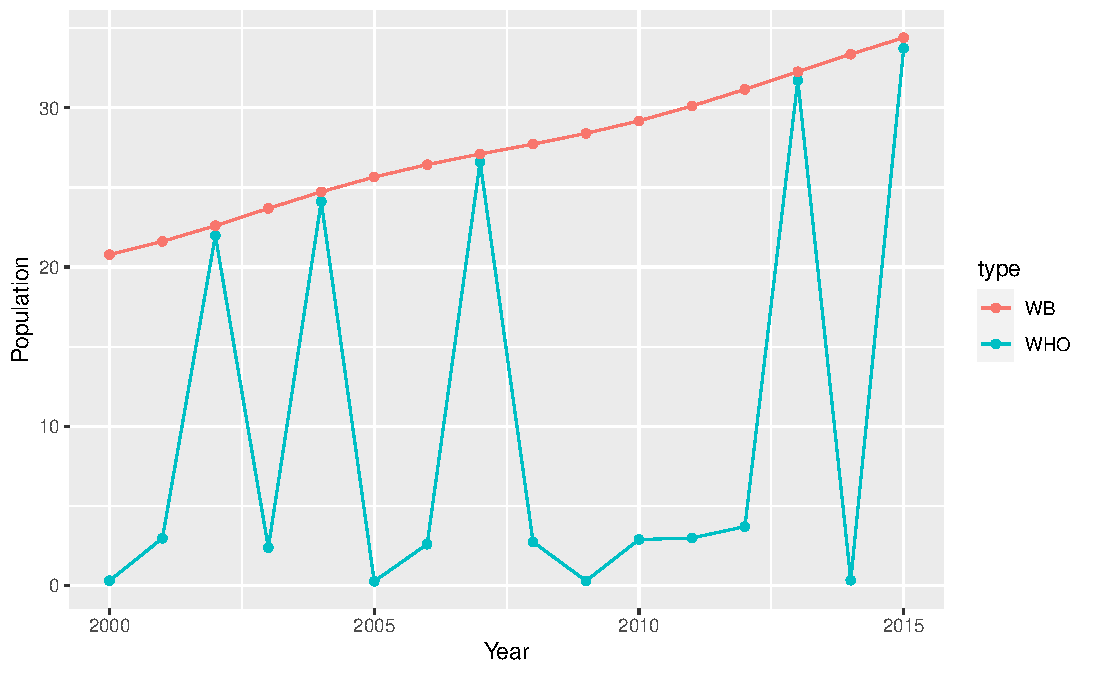
\includegraphics[width = 0.9\textwidth]{figures/Afghanistan_population_comparison}
  \caption{Afghanistan population: comparison of WHO and WB data}
  \label{fig:afghanistan_pop_comparison}
\end{figure}

Almost the same can be said also about the GDP field. The Cook Islands, Monaco, Niue, Papua New Guinea, Saint Kitts and Nevis, San Marino, and Sao Tome and Principe was missing values in one year. Eritrea, Iraq, and Libya were missing four values per each country. South Sudan and Syrian Arab Republic were missing eight values and 26 other countries (including UK) did not have any information at all. As a result, the data table from Global Health Data Exchange (GHDx) database \cite{GHDx} was selected for use for all countries for consistency.

As shown in table \ref{tab:missing}, there were also missing values in some other fields, but not a lot. Since data cleaning was not the main part of this project, a decision was made to simply drop the 26 affected rows.


% \subsection{Variables' Transformation}
% \label{sec:vari-transf}



% ## data description

% ## data cleaning


%%% Local Variables:
%%% TeX-master: "main"
%%% End:

\section{Modeling}
\label{sec:modeling}

This section describe how the best fitting models to predict the Life.expectancy were created. The pre-processed and cleaned dataset contained 157 observations and 23 variables to be considered for the regression model. Three columns: X, Country, and Year, were removed from the pre-processed dataset. Some transformations were applied to produce a better model for predicting the Life.expectancy in 2014 worldwide.

\subsection{Method overview}

In this subsection, the methods used to complete the modeling will be introduced. Multilinear regression, stepwise regression, user-defined variable transformation, and the Variance Inflation Factors (vif) were utilized to produce models in rstudio.

Multilinear regression is an extended regression of simple linear regression. It provides more functionality to support predictions of the response variable with multiple regressors. In R, the mlr function usually is used with the summary function to display the overall quality of the selected model. In the subsequent subsections, the implementation of stepwise regression, variable transformation, and vif function in the modeling process will be described.

Additionally, as the first regression model with all predictors, an Adjusted R-squared: 0.8615, F-statistic: 52.08 and p-value: $< 2.2\times 10^{-16}$ was obtained by executing the r code below:

\begin{verbatim}
summary(lm(Life.expectancy ~ ., data = Dat))
\end{verbatim}

According to the R output, not all regressors are significant enough to contribute to the prediction model. Thus, in the following steps, various methods to improve the Adjusted R-squared score were attempted based on the knowledge and techniques learned in the STAT 5020 course.

\subsection{Data Transformation}

\begin{figure}
  \centering
  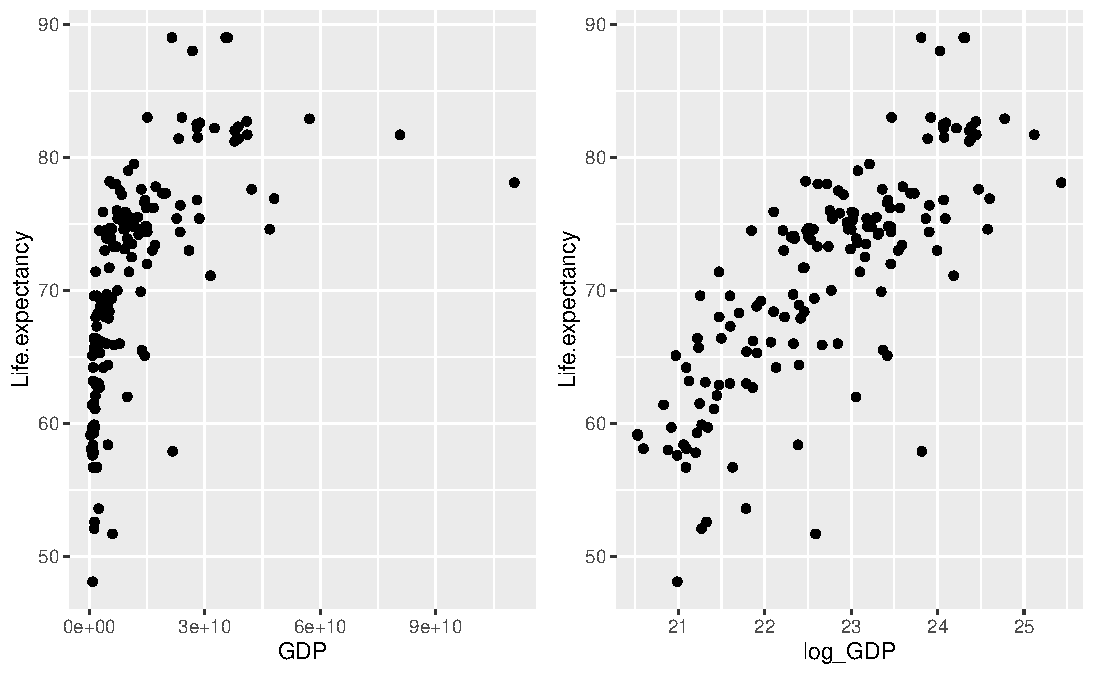
\includegraphics[width = 0.8\textwidth]{figures/transforms}
  \caption{Scatter plots of the GDP vs Life.expectancy variable before and after the transformation}
  \label{fig:transforms}
\end{figure}

In this subsection, the transformations applied to the dataset is described in detail. The GDP distribution before and after the log transformation is shown in figure \ref{fig:transforms}. The transformed function is created by the R code shown below:
\begin{verbatim}
transform <- function(x, scale) {
  if(scale == 0) return(log(1 + min(x) + x))
  else return(x^scale)
}
\end{verbatim}
The function takes two arguments, x as the original input value, and scale as the scaling value to be determined. A condition option for the user to choose when scale equals 0, the original input will be calculated as log(1 + min(x) + x); when the scale is given as a number that does not equal to 0, then the transformed input will be $x^{scale}$.



The transformations were applied as follows: log\_infant.deaths, log\_percentage.expenditure, log\_Measles, log\_under.five.deaths, log\_GDP, and log\_Population.

\begin{verbatim}
model2 <- lm(Life.expectancy ~ ., data = Dat2)
\end{verbatim}

The Adjusted R-squared: 0.8775, F-statistic: 59.83 and p-value: $< 2.2\times 10^{-16}$ was obtained from the new model on the new transformed dataset Dat2.

\subsection{Variance Inflation Factors}

The next step was to use the Variance Inflation Factors to check for multiple collinearity. This step was repeated several times to reduce multicollinearity from the model. The variable Hepatitis.B, log\_GDP, log\_Population, thinness.5.9.years, Income.composition.of.resources, and Schooling were removed. More details are provided in the evaluation section.


\begin{verbatim}
Dat3 <- Dat2[,-c(7, 15, 16, 18, 19, 20)]
model3 <- lm(Life.expectancy ~ ., data = Dat3)
\end{verbatim}
The new model showed the Adjusted R-squared: 0.7849, F-statistic:  44.8, and p-value: $< 2.2\times 10^{-16}$.


\subsection{Stepwise modeling}

The stepwise model selection approach is a way to iteratively add and/or remove candidate variables to build a subset of variables in the provided dataset for a better model. Stepwise regression includes forward, backward, and bidirectional methods. The bidirectional method was selected for this project for more flexible and appropriate models. The key R code to apply this step is listed below. Note the column "Status" is a binary categorical field, so it was converted the text values and assigned 1 for Developed and 0 for Developing.

\subsection{Bidirection model optimization}

\begin{verbatim}
DatSw <- Dat2
DatSw$Status <- ifelse(Dat$Status == "Developing", 0, 1)
stepwise(DatSw, "Life.expectancy", selection = "bidirection", select = "adjRsq")
\end{verbatim}

The library(StepReg), contains stepwise as a built-in function that provides the functionalities for the user to choose the direction to select the predictors, as well as the criterion. "adjRsq" as adjusted R squared is used to determine if the model improves with the addition or removal of a variable. During this step, variates "Adult.Mortality", "Alcohol", "log\_under.five.deaths", "HIV.AIDS","log\_percentage.expenditure", "Status", "Total.expenditure", "log\_infant.deaths", "Diphtheria", "BMI" and "thinness..1.19.years" were selected by the order of the improvement of "adjRsq".

\begin{verbatim}
DatSw <- select(Dat3_, c("Life.expectancy", sw$variate[-1]))
modelSw <- lm(Life.expectancy ~ ., data = DatSw)
\end{verbatim}

The model showed the Adjusted R-squared:  0.7876, F-statistic: 53.59 and p-value: $< 2.2\times 10^{-16}$. The adjusted R squared is expected to decrease since fewer variables were used in the current fitted model.

To optimize the model further, use of the vif function and methods to remove outliers were applied. Details will be provided separately in the Evaluation section. 

\subsection{Interactions}

% latex table generated in R 4.0.3 by xtable 1.8-4 package
% Thu Dec  9 18:45:49 2021
% latex table generated in R 4.0.3 by xtable 1.8-4 package
% Thu Dec  9 18:50:34 2021
% latex table generated in R 4.0.3 by xtable 1.8-4 package
% Thu Dec  9 18:51:17 2021
\begin{table}[ht]
\centering
\begin{tabular}{rlrr}
  \hline
 & v1v2 & $\Delta R^2$ & $\Delta adjR^2$ \\ 
  \hline
1 & Adult.Mortality*HIV.AIDS & 0.01650 & 0.01640 \\ 
  2 & Adult.Mortality*log\_under.five.deaths & 0.00680 & 0.00590 \\ 
  3 & Status*Diphtheria & 0.00680 & 0.00590 \\ 
  4 & Adult.Mortality*Total.expenditure & 0.00680 & 0.00580 \\ 
  5 & Adult.Mortality*log\_infant.deaths & 0.00660 & 0.00570 \\ 
   \hline
\end{tabular}
\caption{Effects of variable interaction} 
\label{tab:int}
\end{table}

Interactions were also a critical aspect to be considered. A simple R function, acting like a forward stepwise function, was written to probe all possible interactions between two variables and take the combination producing the largest increase for the adjusted R2 metric. In table \ref{tab:int} the best 5 best variants are shown and it is evident that  Adult.Mortality*HIV.AIDS should be used. As a result, the final model is defined as
\begin{verbatim}
final_model <- lm(Life.expectancy ~ 
   Alcohol + log_percentage.expenditure + Status + Total.expenditure 
   + Adult.Mortality*HIV.AIDS, data <- DatSw)
\end{verbatim}

An Adjusted R-squared of 0.804 was obtained with the added interaction in the model. After removing the variables that were not significant, an Adjusted R-squared of 0.7959, F-statistic: 87.89 and p-value: $< 2.2\times 10^{-16}$ were obtained. The last step to build the model is look for outliers and other high leverage points and will be explained in the Evaluation section separately.
% The final model we got is shown below with the Adjusted R-squared 0.7959, F-statistic 87.89, and the p-value $< 2.2\time 10^{-16}$. We are satisfied with this model as it gives a good Adjusted R-squared as well as a relatively acceptable number of predictors in the model.

% \begin{verbatim}
% model_cleaned <- lm(
%   Life.expectancy ~  Alcohol + log_percentage.expenditure + Status +
%    Total.expenditure + Adult.Mortality*HIV.AIDS
% , data = Dat_cleaned)
% \end{verbatim}

%%% Local Variables:
%%% TeX-master: "main"
%%% End:

\section{Evaluation}
\label{sec:evaluation}

\subsection{Multicollinearity}
\label{sec:multicollinearity}
Multicollinearity among the regressor variables was checked and those with high variable inflation factor or VIF were removed. The VIF of a variable is the ratio of the variance of the overall model to the variance of a model with only that variable. A VIF greater than 4 indicates moderate multicollinearity and a VIF greater than 10 indicates severe multicollinearity. The regressor variables of Hepatitis.B, transformed logGDP, logPopulation, thinness.5.9.years, Income.composition.of.resources, and, Schooling were removed because they had greater than 4 VIF, and their p-value in the model summary indicated lower significance. 
After removing these variables, the model was fitted and again the VIF and the Pearson correlation coefficients for the variables were calculated. The regressor variables: log\_under.five.deaths, and log\_infant.deaths again had very high VIF and these were taken care of later while considering the interactions between the regressors.

\subsection{Identification of Influential Points}
\label{sec:influential-points}
Further, the points that play an important role than others in determining the regression line were found. High leverage points were looked for by finding fitted values that were greater than 2* (k+1)/n, where k is the number of variables in the model and n is the number of observations used to create the model. The outliers were searched by identifying where the absolute internally studentized and externally studentized residuals are greater than 3. Then, three methods were used to identify potentially influential points. The first method that was used is Difference in Fits, or DFFITS, which is a measure of the difference in fitted values when a chosen observation is removed from the model. A point was considered influential if the absolute value of $DFFITS_i$ was greater than $2* \sqrt{(k+2)/(n-k-2)}$. The second method that was used was Cook’s distance, $D_i$, which identifies influential points by determining which observations had high leverage or were outliers. An observation was considered possibly influential if the value returned from the R function: \textit{cooks.distance()} was greater than 1. The third method used was COVRATIO. An observation was considered possibly influential if the value of $COVRATIO_i$ was greater than $1+ 3*((k+1)/n)$, or less than $1- 3*((k+1)/n)$.
About 7\% of the data points were removed that were overlapping in influential, high leverage, and outlier observations.

\section{Assumptions of a Linear model}
\label{sec:assumptions}

\subsection{Linearity between Explanatory and Response variables}
\label{sec:linearity}
As can be seen from the plots of residual errors again the regressor variables shown in the figure \ref{fig:linearity}, there is not much of a pattern and they are mostly scattered. If these plots are scanned from left to right by considering thin vertical strips, in each strip, the vertical average of the residuals is mostly zero except for Alcohol and Adult mortality. So the assumption about the linearity of our model is satisfied. 

\begin{figure}
  \centering
  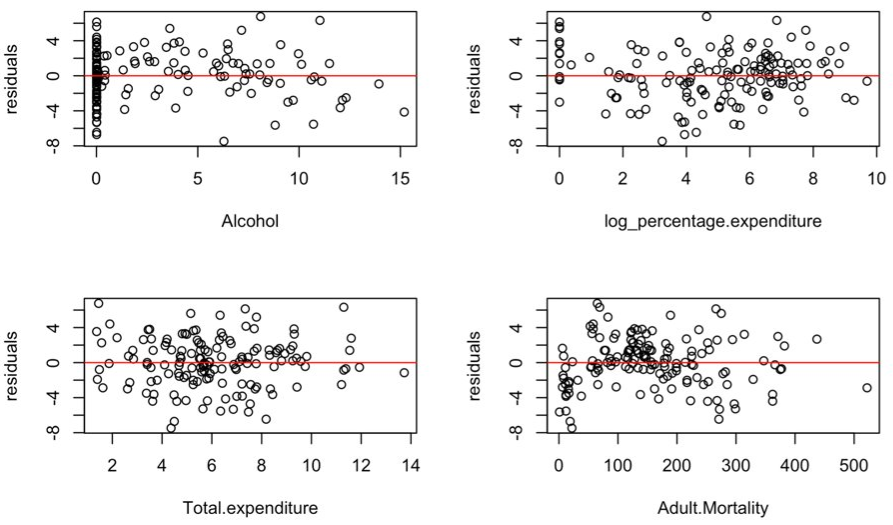
\includegraphics[width = 0.9\textwidth]{figures/linearity.PNG}
  \caption{Residual errors against the regressors}
  \label{fig:linearity}
\end{figure}

\subsection{Independence of Error Terms}
\label{sec:independence}
In the figure \ref{fig:independence}, the residual errors are plotted against the row numbers sorted by regressor variables for checking the independence of error terms assumption. As these plots are scanned from left to right by considering thin vertical strips, it is noticed that they are randomly and symmetrically distributed around zero. Hence, it is concluded that our model passed the assumption of independence of error terms. 

\begin{figure}
  \centering
  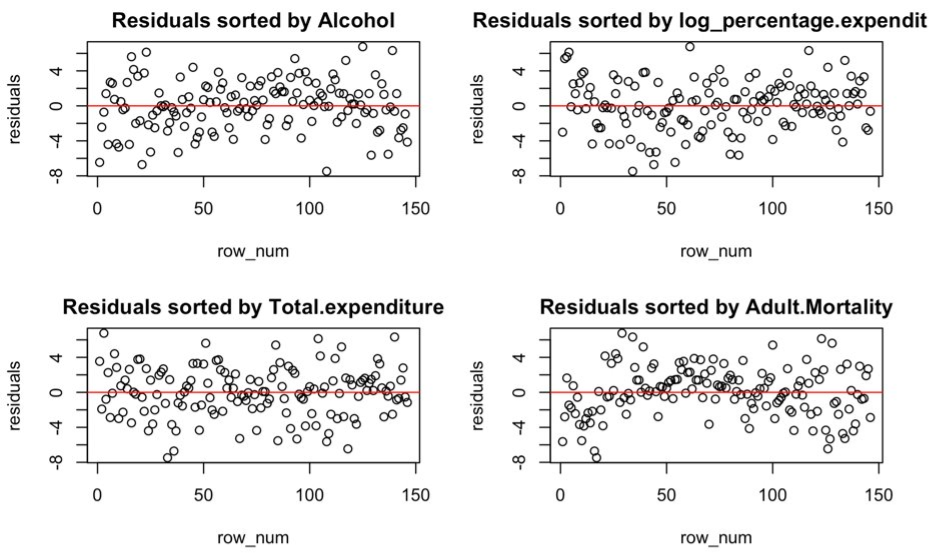
\includegraphics[width = 0.9\textwidth]{figures/independence.PNG}
  \caption{Residuals against the row numbers sorted by regressors}
  \label{fig:independence}
\end{figure}

\subsection{Normality in the Distribution of Error Terms}
\label{sec:normality}

\begin{figure}
  \centering
  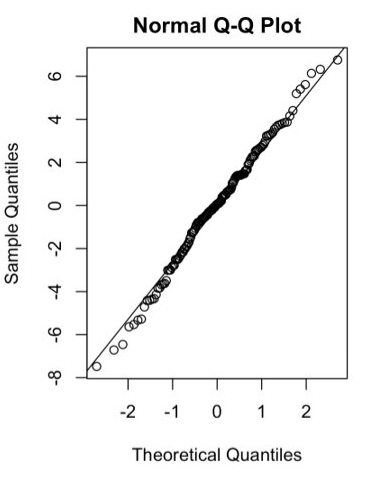
\includegraphics[width = 0.45\textwidth]{figures/normality.PNG}
  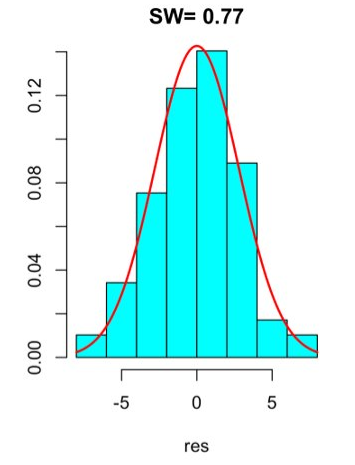
\includegraphics[width = 0.45\textwidth]{figures/Shapiro.PNG}
  \caption{Normal Q-Q plot}
  \label{fig:normality}
\end{figure} 


As can be seen from the left panel of figure \ref{fig:normality} showing the Q-Q plot, the points approximately fall on a straight line, which supports the assumption of normality between error terms.


The Shapiro-Wilk test was also conducted to check for the normal distribution of the error terms where the null hypothesis is that the errors follow a normal distribution. As shown in the right panel of  figure \ref{fig:normality}. The p-value obtained from the test was 0.77 which is greater than the \textit{alpha} of 0.05. Hence, we failed to reject the null hypothesis and thus it was found that the error terms follow the normal distribution. 




%%% Local Variables:
%%% TeX-master: "main"
%%% End:


\section{Conclusion}
\label{sec:conclusion}

The initial model obtained with the inclusion of all variables including log transformations of select variables produced an Rsquared value of 0.89. The final model contained significantly fewer variables and gave an Rsquared value of 0.86. This small reduction in the Rsquared value is a small price to pay to reduce the complexity of the model.

Table 4 contains the relevant variables of the final model. The final model equation is:

\begin{verbatim}
hat(LE) = 73.1 + 0.3126 Alcohol + 
       0.4845 log_percentage.expenditure + 
       3.0819 Status + 0.3619 Total.expenditure - 
       0.0436 Adult.Mortality - 3.9860 + 0.0080 Adult.Mortality*HIV.AIDS
\end{verbatim}



% latex table generated in R 4.0.3 by xtable 1.8-4 package
% Fri Nov 26 11:47:04 2021
\begin{table}[ht]
\centering
\begin{tabular}{@{}p{0.1\linewidth}  p{0.3\linewidth}p{0.5\linewidth}p{0.1\linewidth}@{}}
  \toprule
 & Variable & Description \\ 
  \midrule

1 & Status & Developed or Developing status \\ 
  2 & Adult Mortality &  Adult Mortality Rates of both sexes (probability of dying between 15 and 60 years per 1000 population) \\ 
  3 & HIV.AIDS &  Deaths per 1 000 live births HIV/AIDS (0-4 years) \\ 
  4 & Percent Expenditure &  Expenditure on health as a percentage of Gross Domestic Product per capita\\ 
  5 & Total Expenditure &  General government expenditure on health as a percentage of total government expenditure \\ 
 6 & Alcohol &  Alcohol, recorded per capita (15+) consumption (in litres of pure alcohol)\\

\bottomrule
\end{tabular}
\caption{Final Model Variables}
\label{tab:missing}
\end{table}

It came as a surprise that GDP was not present in the final model, but upon further investigation of the detailed description of the variables, it can be seen that GDP is encapsulated in the "Percent Expenditure" variable. 

With much attention paid to life expectancy over the last 100 years or so, there has been a two-fold increase in life expectancy worldwide. Differences do exist between countries of the world and can even be seen in various regions within countries. Government policies, the wealth of a country, and habits of the population can certainly influence the longevity of a population. The current COVID-19 pandemic certainly showcases the gap in resources between countries and their public health policies. 

While this particular model only considered one particular year in time, further study is necessary to determine if the model is valid over multiple years. It is also possible that with the current global pandemic, the world will experience a decline in the average life expectancy.




% ## adjusted r^2 

%%% Local Variables:
%%% TeX-master: "main"
%%% End:

% # reference

\let\Section\section 
\def\section*#1{\Section{#1}} 
\bibliographystyle{alpha}
\bibliography{refrences}

\end{document}

